\def\year{2017}
 \documentclass[letterpaper]{article}
 \usepackage{aaai}
 \usepackage{times}
 \usepackage{helvet}
 \usepackage{courier}
 \setlength{\pdfpagewidth}{8.5in} 
 \setlength{\pdfpageheight}{11in}

%\usepackage[pdftex]{graphicx}
% \graphicspath{{../pdf/}{../jpeg/}}
\usepackage{url}

%MARTA HEADER begin
\usepackage{tikz}
\newenvironment{mmm}[2]{{#1}}{}
%\newenvironment{mmm}[2]{{\bf \color{blue} #1}{\color{red} #2}}{}

%MARTA HEADER end

% correct bad hyphenation here
\hyphenation{op-tical net-works semi-conduc-tor}

\begin{document}
\title{TransportEditor -- Creating and Visualising Transportation Problems and Plans}

%\author{Paper \#92}
 \author{Ondrej \v{S}kopek and Roman Bart\'{a}k \\
 Charles University, Faculty of Mathematics and Physics \\
 Malostransk\'{e} n\'{a}m. 25, Praha 1, Czech Republic}


\maketitle

\begin{abstract}
\begin{quote}
Transportation planning became a popular domain for automated planning systems and many domains in International Planning Competitions involve some form of a transportation problem. This paper introduces \emph{TransportEditor} -- a Java program for creating various variants of transportation domain models, for editing and visualising specific problem instances, for generating a plan by calling external or internal planners, for validating the plans for example by VAL, and finally for visualising and tracing the plans.
\end{quote}
\end{abstract}

\section{Introduction}
Automated planning struggles from the lack of tools for editing and visualising planning domain models and plans. This is partly due to generality of the concept of automated planning, that makes it hard to develop general editors while covering peculiarities of a specific domain, and partly due to less interest in knowledge engineering aspects of planning. There exists only a few generally applicable tools such as itSimple \cite{itsimple}, GIPO \cite{gipo}, and Planning.Domains \cite{pd}, PDDL editors such as PDDL Studio \cite{studio} and VIZ \cite{viz} and plan visualisers such as iGantt \cite{igantt} and VisPlan \cite{visplan}.

In this system demo we introduce \emph{TransportEditor} --  a Java program for working with transportation planning domains that appear in various flavours in International Planning Competitions (IPC).

\section{Transport Domain}
Transport domain has been introduced in IPC 2008 and it deals with transporting packages between locations using trucks. There is a directed graph defining locations and connections between them. Edges might be weighted to model distance, time or fuel consumption for moving between locations. Packages are initially waiting at some locations (nodes) and the goal is to deliver them to their destination locations using trucks. The trucks are also initially waiting at certain locations so they may need to drive to pick up packages. The package must be loaded to a truck before it can be transported, and it must de unloaded to get to a specific location. Trucks may have limited capacity described by the number of packages that they can transport at the same time. The trucks may also consume fuel during transportation and they may need to refuel at certain locations.

In addition to being a classical real-life domain that is also known as a vehicle routing problem, the flavour of the Transport domain can be found in many other IPC domains including Nomystery, Childsnack, Tidybot, Logistics, Depots, and DriverLog,  among others. Hence we believe that it is important to have a visual environment for problem specification and plan visualisation devoted specifically to transportation problems. The goal is to simplify human understanding of specific problem instances and plans for them by visualising both the problem instances and the plans in an integrated form. 


\section{Domain and Problem Editing}
The TransportEditor supports both sequential and temporal planning domain models. The major difference is that the temporal model includes durative actions and supports concurrent actions. In both cases, it is possible to assume limited capacity of trucks as well as fuel consumption for driving and refuelling actions. The system can load the existing PDDL domain model for the Transport domain or the user may create a new domain model simply by selecting the required properties. This is useful to design versions of the domain model for a specific planner that supports only a subset of the domain model features.

The second step after having the domain model is specifying the problem instance. Again, the system allows loading the problem instance from the PDDL file (and then editing it) or creating it from scratch. We will describe the most general properties of objects in the instance, some of them might not be available for particular domain models. Basically, there are four types of objects in the transport domain: locations, connections, packages, and trucks. For each location, the user may specify its (X,Y) coordinate and indicate whether a refuelling station is available at that location. Connection must always lead from one location to another location and it may be parameterised by length and fuel consumed when driving between the locations. Locations and connections define a directed graph that is visualised by the software. The user has the freedom to place the nodes (locations) anywhere in the 2D area, the system tries (on demand) to display the graph in a visually pleasant way.

The other two types of objects in the domain are trucks and packages. For each package the user specifies its current location and its destination location and also its size to be used if trucks have limited capacity. For each truck, it is possible to specify its current and destination locations, as well as capacity (current and maximal) for packages and for fuel.

Figure~\ref{fig:editor} shows the TransportEditor when displaying a particular problem instance on the left panel. Domain models and problem instances can be saved in PDDL so they can be used by any PDDL-compliant planner.

\begin{figure}[]
        \centering
        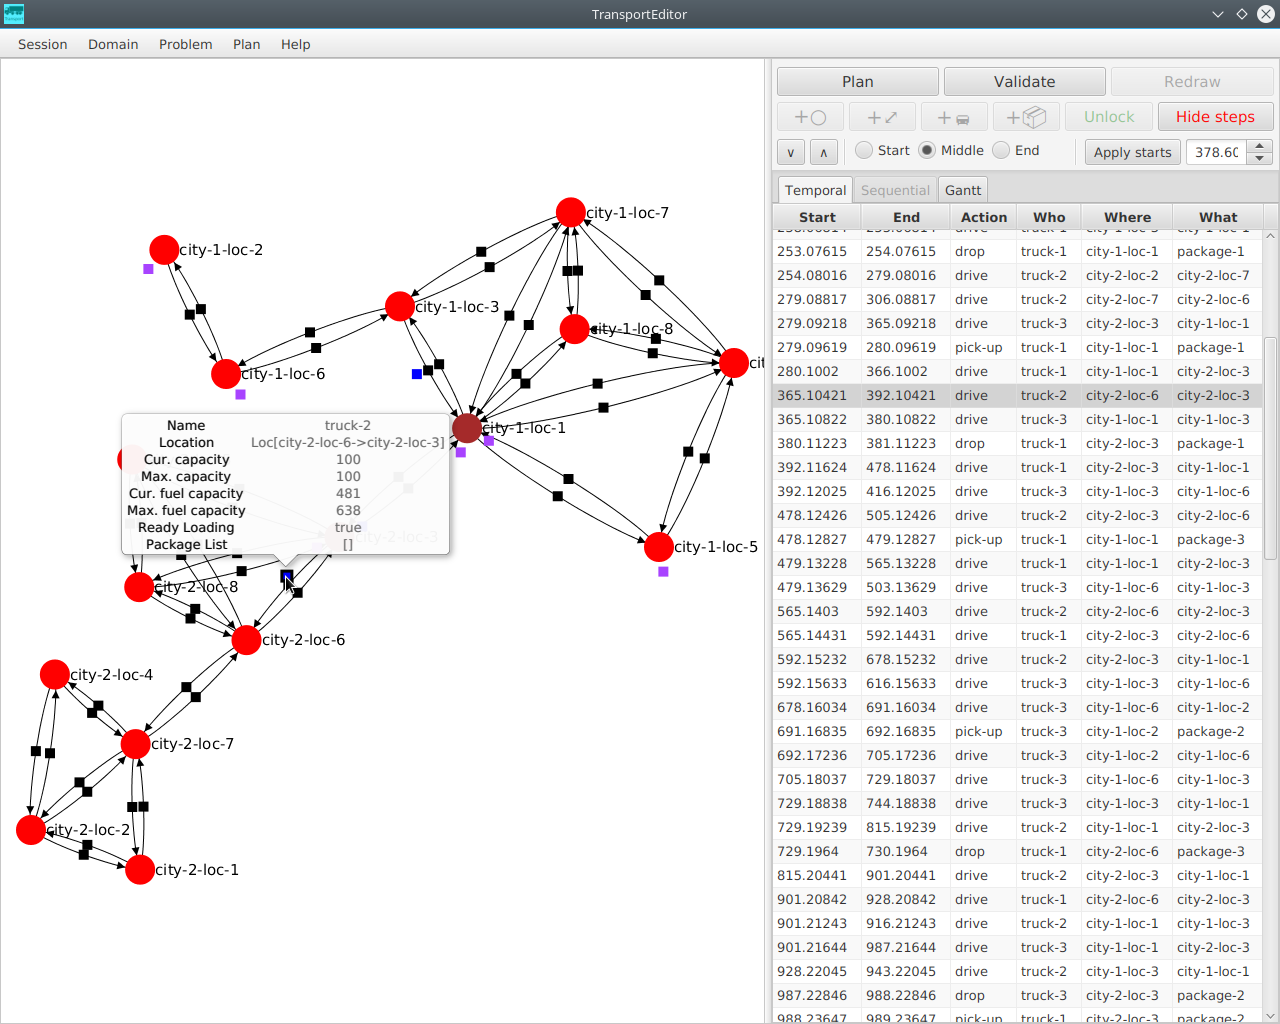
\includegraphics[width=0.45\textwidth]{editor.jpg}
        \caption{TransportEditor showing an instance of the planning problem (left) wit locations of packages (violet squares)  and trucks (blue squares) and a particular temporal plan (right).}
    \label{fig:editor}
\end{figure}

\section{Planning}
The TransportEditor has its own build planners that can be applied to currently opened problem instance (based on DFS and A*) but the user can use any installed domain-independent planner that accepts domain models and problem instances in PDDL. It is only necessary to specify the command line to call the planner.


\section{Plan Visualisation, Validation, and Tracing}
The final step in using the TransportEditor is visualising the plans, their validation, and dynamic tracing. The system can open the plan produced by an external planner and show it as a (time annotated) sequence of actions. It is also possible to display the plan in the form of a Gantt chart that makes it easier to spot concurrent actions for temporal planning. The plan can also be validated, for example by calling VAL \cite{val}. Again, this is done by specifying the command line to call the validator. In addition to static visualisation of the plan, it is possible to trace it and to observe locations of trucks and packages in any step of the plan (see the right panel of Figure~\ref{fig:editor}).


\section{Summary}
Transportation planning is an important real-life problem and a challenging benchmark for automated planners. TransportEditor attempts to simplify development of planning domain models with various constraints by visualising particular problem instances and plans and connecting planners and validators to simplify the workflow for human developers. The tool is implemented in Java so it is accessible for various computer platforms.


% no keywords
% use section* for acknowledgment
\subsection*{Acknowledgments}
Roman Bart\'{a}k is supported by the Czech Science Foundation under the project P103-15-19877S.



\begin{thebibliography}{}

\bibitem[\protect\citeauthoryear{Bart\'{a}k and Skalick\'{y}}{2009}]{igantt}
R. Bart\'{a}k, T. Skalick\'{y}. A local approach to automated correction of violated precedence and resource constraints in manually altered schedules. In \emph{Proceedings of MISTA 2009: Fourth Multidisciplinary International Scheduling Conference: Theory and Applications}, Dublin, Ireland, pp. 507--517, 2009.

\bibitem[\protect\citeauthoryear{Muise}{2016}]{pd}
C. Muise. Planning.domains. In \emph{ICAPS system demonstration}, 2016.

\bibitem[\protect\citeauthoryear{Howey and Long}{2003}]{val}
R. Howey and D. Long. VAL's Progress: The Automatic Validation Tool for PDDL2.1 used in the International Planning Competition. In \emph{Proceedings of the ICAPS 2003 workshop on "The Competition: Impact, Organization, Evaluation, Benchmarks"}, June 2003, Trento, Italy.

\bibitem[\protect\citeauthoryear{Glinsk\'{y} and Bart\'{a}k}{2013}]{visplan}
R. Glinsk\'{y}, R. Bart\'{a}k. VisPlan -- Interactive Visualisation and Verification of Plans. In \emph{ICAPS system demonstration}, 2013.

\bibitem[\protect\citeauthoryear{Plch et al.}{2012}]{studio}
Tom\'{a}\v{s} Plch, Miroslav Chomut, Cyril Brom, Roman Bart\'{a}k. Inspect, Edit and Debug PDDL Documents: Simply and Efficiently with PDDL Studio. In \emph{ICAPS system demonstration}, 2012.

\bibitem[\protect\citeauthoryear{Simpson et al.}{2007}]{gipo}
R.M. Simpson, D.E. Kitchin, T.L. McCluskey. Planning Domain Definition using GIPO. \emph{The Knowledge Engineering Review} 22(2): 117--134, 2007.

\bibitem[\protect\citeauthoryear{Vaquero et al.}{2013}]{itsimple}
T. S. Vaquero, J. R. Silva, F. Tonidandel, and J. C. Beck. itSimple: towards an integrated design system for real planning applications. \emph{Knowledge Engineering Review}, 28(2):215--230, 2013.

\bibitem[\protect\citeauthoryear{Vodr\'{a}\v{z}ka and Chrpa}{2010}]{viz}
J. Vodr\'{a}\v{z}ka, L. Chrpa. Visual design of planning domains. In \emph{Proceedings of KEPS 2010: Workshop on Knowledge Engineering for Planning and Scheduling}, ICAPS 2010, Toronto, Canada, pp. 68--69, 2010.

\end{thebibliography}


% that's all folks
\end{document}

